%%%%%%%%%
% SETUP %
%%%%%%%%%

\documentclass{beamer}
\mode<presentation> {
	\usetheme{Madrid}
}
\setbeamertemplate{frametitle continuation}[from second][]

\usepackage{graphicx}
\usepackage{booktabs}

\usepackage{tikz}
\usetikzlibrary{knots}
\usetikzlibrary{arrows.meta} 

% Title.
\title[The Banach--Tarski Paradox and Amenability]{The Banach--Tarski Paradox and Amenability}
\author{Daniel Dunmore}
\institute[UNSW]{
	University of New South Wales \\
	\medskip
	\textit{d.dunmore@unsw.edu.au}
}
\date{\today}

% Bibliography.
\usepackage[%
	backend = biber,
	% BibLaTeX-Math package: https://github.com/konn/biblatex-math
	style = math-alphabetic,
	giveninits = true,
	dashed = false,
	url = false,
	doi = false,
	sorting = none,
	minalphanames = 3,
	maxalphanames = 4
]{biblatex}
% Use the default font size for the bibliography.
\renewcommand*{\bibfont}{\normalsize}
% Use title case rather than sentence case for references.
\DeclareFieldFormat{titlecase}{#1}
% Put last names before first names.
\DeclareNameAlias{default}{family-given}
% Used for articles with appendices written by other authors.
\NewBibliographyString{bywithappendix}
\DefineBibliographyStrings{english}{
	bywithappendix = {with an appendix by}
}
% Specify the bibliography data file to use.
\addbibresource{References.bib}
% Sort by order present in .bib file.
\nocite{*}


%%%%%%%%%%%%
% NOTATION %
%%%%%%%%%%%%

\usepackage{mathrsfs}

% Adds integral notation like \oiint.
\usepackage{esint}
% Blackboard bold symbols.
\usepackage{bbm}

\usepackage{accents}
% Tilde notation for vectors.
\newcommand{\ut}[1]{\underaccent{\tilde}{#1}}
% Arrow notation for vectors.
\usepackage{harpoon}
% Dirac bra-ket notation for quantum states.
\usepackage{braket}

% Differential formatting.
\usepackage{ifthen}
\usepackage{etoolbox}
\newcommand*{\ndiff}[1]{\mathrm{d}#1}
\newcommand*{\sdiff}[1]{\mathop{}\!\ndiff{#1}}
\newcommand{\rdiff}[3][]{
	\ifthenelse{\equal{#1}{}}
	{\frac{\mathrm{d}#2}{\mathrm{d}#3}}
	{\frac{\mathrm{d}^{#1}#2}{\forcsvlist\ndiff{#3}}}
}
\newcommand*{\npiff}[1]{\mathrm{\partial}#1}
\newcommand*{\spiff}[1]{\mathop{}\!\npiff{#1}}
\newcommand{\rpiff}[3][]{
	\ifthenelse{\equal{#1}{}}
	{\frac{\mathrm{\partial}#2}{\mathrm{\partial}#3}}
	{\frac{\mathrm{\partial}^{#1}#2}{\forcsvlist\npiff{#3}}}
}
% Inexact differential for physics.
\newcommand*{\dbar}[1]{\mathop{}\!\mathrm{\dj}#1}

% Metrics, inner products and norms.
\usepackage{mathtools}
\DeclarePairedDelimiter{\abs}{\lvert}{\rvert}
\DeclarePairedDelimiter{\inprod}{\langle}{\rangle}
\DeclarePairedDelimiter{\norm}{\lVert}{\rVert}
% This is used if we want an empty norm. 
\newcommand{\blank}{{}\cdot{}}

% Function notation.
\newcommand{\id}{\mathrm{id}}
\newcommand{\coker}{\mathrm{Coker}}
\newcommand{\im}{\mathrm{Im}}
\newcommand{\ev}{\mathrm{ev}}
\newcommand{\coev}{\mathrm{coev}}

% Category theory notation.
%\newcommand{\obset}{\textnormal{Ob}_{#1}\!\left(#2\right)}
%\newcommand{\morset}[2][]{\textnormal{Mor}_{#1}\!\left(#2\right)}
%\newcommand{\homset}[2][]{\textnormal{Hom}_{#1}\!\left(#2\right)}
%\newcommand{\End}[2][]{\textnormal{End}_{#1}\!\left(#2\right)}
%\newcommand{\opp}[1]{{#1}^{\textnormal{op}}}
%\newcommand{\textcat}[1]{\textnormal{\textsf{#1}}}
\newcommand{\obset}{\mathrm{Ob}}
\newcommand{\morset}{\mathrm{Mor}}
\newcommand{\homset}{\mathrm{Hom}}
\newcommand{\End}{\mathrm{End}}
\newcommand{\opp}{\mathrm{op}}
\newcommand{\textcat}[1]{\mathrm{\textsf{#1}}}
\newcommand{\textobj}[1]{\mathrm{\texttt{#1}}}

% Special notation.
%\newcommand{\chr}{\textnormal{char}}
%\newcommand{\Tr}{\textnormal{Tr}}
%\newcommand{\trv}{\textnormal{tr}}
%\newcommand{\Dim}{\textnormal{Dim}}
%\newcommand{\FPdim}{\textnormal{FPdim}}
\newcommand{\chr}{\mathrm{char}}
\newcommand{\Tr}{\mathrm{Tr}}
\newcommand{\trv}{\mathrm{tr}}
\newcommand{\Dim}{\mathrm{Dim}}
\newcommand{\FPdim}{\mathrm{FPdim}}

% Hiragana "yo" for the Yoneda embeddings.
\newcommand{\yo}{\text{\usefont{U}{min}{m}{n}\symbol{'210}}}
\DeclareFontFamily{U}{min}{}
\DeclareFontShape{U}{min}{m}{n}{<-> udmj30}{}

% Representation theory notation.
\newcommand{\Sym}{\mathrm{Sym}}
\newcommand{\Alt}{\mathrm{Alt}}

\usepackage{calc}

\newcommand*{\emphasis}[1]{\textcolor{structure}{\em #1}}

\usefonttheme[onlymath]{serif}

\DeclareCiteCommand{\aycite}
{\boolfalse{citetracker}\boolfalse{pagetracker}}
{\printtext[bibhyperref]{\printnames{labelname}\addcomma\addspace\printfield{year}}}
{\multicitedelim}
{}

% Negative horizontal phantom.
\newcommand{\nhphantom}[1]{\sbox0{#1}\hspace{-\the\wd0}}

\newtheorem{proposition}{Proposition}
\newtheorem{theoremdefinition}{Theorem-Definition}

\usepackage{stmaryrd}

\renewcommand*{\bibfont}{\normalfont\footnotesize}


%%%%%%%%%%%%
% DOCUMENT %
%%%%%%%%%%%%

\begin{document}

%%%%%%%%%%%
% Prelude %
%%%%%%%%%%%

\begin{frame}
\noindent\\[-20pt]
\begin{figure}[!ht]
\titlepage
\noindent\\[-20pt]
\hspace{3.5cm}\hfill
\includegraphics[width=2cm]{unsw-crest}\hfill\raisebox{-0.7093cm}{
\includegraphics[width=3.5cm]{QR}}
\end{figure}
\end{frame}

\begin{frame}
\frametitle{Today's Story}
\noindent The main goal of my talk today will be to explain the famous Banach--Tarski paradox, first described in 1924.\\[\baselineskip]%\cite{BT24}.\\[\baselineskip]

\noindent This ``veridical paradox'' (to use the terminology of Quine) is in fact the middle child in a triplet of ``paradoxes'' from the early 1900s, with its elder and younger siblings being the Hausdorff paradox (1914) and the von Neumann paradox (1929), respectively.\\[\baselineskip]%(\cite{Hau14}) and the von Neumann paradox (\cite{Neu29}), respectively.\\[\baselineskip]

\noindent If there's enough time, I would then like to give an overview of the surprising impact it has had via the notion of amenability.
\end{frame}

%\begin{frame}
%\frametitle{Today's Story}
%\noindent To give some initial perspective, let's spoil the ``punchline'' of this talk.\\[0.5\baselineskip]

%\begin{theorem}[Tarski's Alternative, 1949]
%A discrete group is amenable if and only if it does \underline{not} admit a paradoxical decomposition.
%\end{theorem}

%\noindent\\[0.5\baselineskip] As is typically the case with stories involving discrete groups, there is a generalization of this result to the world of locally compact groups. We will stay within the realm of the discrete for the sake of simplicity.
%\end{frame}

\begin{frame}
\frametitle{Roadmap}
\begin{center}
\begin{minipage}{\widthof{(4) Representation Theory:\ Categorified}}
\setlength{\parskip}{4ex}
\tableofcontents
\end{minipage}
\end{center}
\end{frame}

%%%%%%%%%%%%%%%%%%%%%%%%%%%%%%
% Paradoxical Decompositions %
%%%%%%%%%%%%%%%%%%%%%%%%%%%%%%

\section{Paradoxical Groups}

\begin{frame}
\frametitle{Paradoxical Decompositions}
\begin{definition}[Paradoxical Decomposition]
Let $G$ be a group and $X$ a $G$-set. We say that the action of $G$ on $X$ is \textbf{$\boldsymbol{G}$-paradoxical} if there exist pairwise disjoint $A_1, \dots, A_n, B_1, \dots, B_m \subseteq X$ and elements $g_1, \dots, g_n, h_1, \dots, h_m \in G$ such that\\[-1.5\baselineskip]
\begin{align*}
\begin{split}
X = \bigcup_{i=1}^n g_i \cdot A_i = \bigcup_{j=1}^m h_j \cdot B_j.
\end{split}
\end{align*}
In this case, $X$ is called a \textbf{$\boldsymbol{G}$-paradoxical set}, and the collection $(A_i, B_j, g_i, h_j)$ is called a \textbf{$\boldsymbol{G}$-paradoxical decomposition} of $X$.
\end{definition}

\noindent\\[0.5\baselineskip] Any group $G$ is itself a $G$-set with respect to, say, left multiplication, so we have a natural notion of groups themselves being paradoxical.\\[\baselineskip]

%\noindent\\[0.5\baselineskip] Note that this is equivalent to the existence of $(A_i, B_j, g_i, h_j)$ such that\\[-1.5\baselineskip]
%\begin{align*}
%\begin{split}
%X = \bigsqcup_{i=1}^n A_i = \bigsqcup_{j=1}^m B_j = \bigsqcup_{i=1}^n g_i \cdot A_i = \bigsqcup_{j=1}^m h_j \cdot B_j.
%\end{split}
%\end{align*}

%\noindent\\[0.5\baselineskip] Any group $G$ is itself a $G$-set with respect to, say, left multiplication, so we have a notion of groups themselves being paradoxical.
\end{frame}

%\begin{frame}
%\frametitle{Paradoxical Decompositions}
%Any group $G$ is itself a $G$-set with respect to, say, left multiplication, so we have a natural notion of groups themselves being paradoxical.\\[\baselineskip]

%In fact, we can push this property of the group onto a set on which it acts using the Axiom of Choice.\\[0.5\baselineskip]

%\begin{theorem}
%A group is paradoxical if and only if it admits a free action on a paradoxical set.
%\end{theorem}
%\end{frame}

\begin{frame}
\frametitle{Paradoxical Decompositions}
\begin{example}[Finite Groups]
A finite group $G$ is \underline{never} paradoxical! This is because we would require\\[-1.5\baselineskip]
\begin{align*}
\begin{split}
\abs{A_1} + \cdots + \abs{A_n} = \abs{G} = \abs{B_1} + \cdots + \abs{B_m},
\end{split}
\end{align*}
\noindent\\[-0.5\baselineskip] which means these subsets cannot be disjoint.
\end{example}
\noindent\\[0.5\baselineskip]
\begin{example}[Abelian Groups]
Abelian groups are also never paradoxical (more on this later).
\end{example}
\noindent\\[0.5\baselineskip]
%\begin{example}[Abelian Groups]
%An Abelian group $G$ is also never paradoxical (this is a bit trickier to show).
%\end{example}
%\noindent\\[0.5\baselineskip]
\begin{example}[Free Groups]
Let $F_2$ be the non-Abelian free group with free generating set $\{a, b\}$. Let $\omega(x)$ be the set of all reduced words in $F_2$ starting with $x$. Then $F_2$ admits the paradoxical decomposition $F_2 = \omega(a) \cup a\cdot\omega(a^{-1}) = \omega(b) \cup b\cdot\omega(b^{-1})$.\\[-1.5\baselineskip]
%\begin{align*}
%\begin{split}
%F_2 = \omega(a) \cup a\omega(a^{-1}) = \omega(b) \cup b\omega(b^{-1}).
%\end{split}
%\end{align*}
\end{example}
%\noindent\\[0.5\baselineskip] This is a particularly important example for the following reason.
\end{frame}

\begin{frame}
\frametitle{Paradoxical Decompositions}
We can in fact push this property of the group onto a set on which it acts using the following theorem, which makes use of the Axiom of Choice.\\[0.5\baselineskip]

\begin{theorem}
If $G$ is a paradoxical group, then any set $X$ that it acts freely on is $G$-paradoxical. %Conversely, if a group $G$ acts freely on a paradoxical\linebreak set $X$, then $G$ is itself paradoxical.
\end{theorem}
\noindent\\[0.5\baselineskip] Moreover, because non-identity subgroups always act freely via left multiplication, we obtain immediately the following result (where the forward direction is of course tautological).\\[0.5\baselineskip]
\begin{corollary}
A group $G$ is paradoxical if and only if it contains a paradoxical subgroup.
\end{corollary}
\noindent\\[0.5\baselineskip] %\textbf{Proof.} The forward direction is tautological. Conversely, if $H$ is a paradoxical subgroup of $G$ with paradoxical decomposition $(A_i, B_j, g_i, h_j)$,\\[-1.5\baselineskip]% then
%\begin{align*}
%\begin{split}
%G = \left(\bigcup_{i=1}^n g_i \cdot A_i\right) \cup (G\setminus H) = \left(\bigcup_{j=1}^m h_j \cdot B_j\right) \cup (G\setminus H),
%\end{split}
%\end{align*}
%\noindent\\[-0.5\baselineskip]giving us the result. \hfill \ensuremath{\blacksquare}\\[\baselineskip]

%Looking for free subgroups is one of the most convenient ways of checking for paradoxical decompositions. For example...%\\[0.5\baselineskip]
%\begin{example}[Braid Groups]
%Any braid group on three or more strands contains $F_2$ as a subgroup, and is hence paradoxical.
%\end{example}
\end{frame}

\begin{frame}
\frametitle{Paradoxical Decompositions}
Looking for free subgroups is one of the most convenient ways of checking for paradoxical decompositions. For example...\\[0.5\baselineskip]
\begin{example}[Braid Groups]
Any braid group on three or more strands contains $F_2$ as a subgroup, and is hence paradoxical.
\end{example}
\noindent\\[0.5\baselineskip]
\begin{example}[3D Rotation Group]
The 3D rotation group $\textup{SO}(3)$ contains $F_2$ as a subgroup, and is hence paradoxical.
\end{example}
%\noindent\\[0.5\baselineskip]
%\begin{example}[2D Rotation Group]
%The 2D rotation group $\textup{SO}(2)$ is Abelian, so it is \underline{not} paradoxical!
%\end{example}
\noindent\\[0.5\baselineskip] Another nice application of our theorem is the paradox of Hausdorff.
\end{frame}

%%%%%%%%%%%%%%%%%%%%%%%%%
% The Hausdorff Paradox %
%%%%%%%%%%%%%%%%%%%%%%%%%

\section{The Hausdorff Paradox}

\begin{frame}
\frametitle{The Hausdorff Paradox}
\begin{theorem}[Hausdorff Paradox, 1914]
There exists a countable subset of the sphere $M \subset S^2$ such that its complement is paradoxical with respect to the canonical action of $\textup{SO}(3)$.
\end{theorem}
%\begin{theorem}[Banach--Tarski Paradox]
%The sphere $S^2$ is paradoxical with respect to the canonical action of $\textup{SO}(3)$.
%\end{theorem}
\noindent\\[0.5\baselineskip] Although one can certainly come up with an explicit $\textup{SO}(3)$-paradoxical decomposition, the fastest way to show this is to find a free action of a free subgroup $F \subset \textup{SO}(3)$.\\[\baselineskip]

\textbf{Proof.} Fix a free subgroup $F$ and let $M$ be the set of all points in $S^2$ that are fixed by $F$. Because $F$ is countable and every non-trivial rotation of $S^2$ fixes two points, $M$ itself is countable. Since $S^2\setminus M$ is invariant under the (free) action of $F$, the result follows from our previous theorem. \hfill \ensuremath{\blacksquare}\\[\baselineskip]

Let's take this a step further.
\end{frame}

%%%%%%%%%%%%%%%%%%%%%%%%%%%%%%
% The Banach--Tarski Paradox %
%%%%%%%%%%%%%%%%%%%%%%%%%%%%%%

\section{The Banach--Tarski Paradox}

\begin{frame}
\frametitle{The Banach--Tarski Paradox}
%Given the existence of fixed points, how are we meant to decompose $S^2$, let alone an entire 3D ball? The answer is by introducing translations.\\[0.5\baselineskip]

\begin{definition}[Equidecomposability]
Let $G$ be a group and $X$ a $G$-set. We say that two subsets $A, B \subseteq X$ are \textbf{$\boldsymbol{G}$-equidecomposable} if there exists a partition $A_1, \dots, A_n$ of $A$, a partition $B_1, \dots, B_n$ of $B$ and $g_1, \dots, g_n \in G$ such that $g_i\cdot A_i = B_i$ for all $i$. This defines an equivalence relation of sets, denoted by $A \sim_G B$.
\end{definition}
%\noindent\\[0.5\baselineskip]
%\begin{proposition}
%If $A$ is paradoxical and $B$ is equidecomposable to $A$, then $B$ is paradoxical.
%\end{proposition}
\noindent\\[0.5\baselineskip]% The proof of this is straightforward and not particularly interesting. We do, however, have the following result.\\[0.5\baselineskip]
%\begin{proposition}
%Let $M$ be a countable subset of $S^2$. Then $S^2$ and $S^2\setminus M$ are $\textup{SO}(3)$-equidecomposable.
%\end{proposition}
\begin{example}[``Reverse Hilbert's Hotel'']
Suppose $A = S^1\setminus\{(1, 0)\}$ and $B = S^1$. Let $g_1$ be the clockwise rotation by $1$ radian, $g_2$ the identity, $A_1 = \{(\cos(n), \sin(n)) : n \in \mathbb{Z}_+\}$ and $A_2 = A\setminus A_1$. Observe that $g_1\cdot A_1 = \{(\cos(n), \sin(n)) : n \in \mathbb{N}\} \eqcolon B_1$ is countably infinite. Thus by taking $B_2 = A_2$, we find that $A \sim_{\textup{SO}(2)} B$.
\end{example}
%\begin{proposition}
%If $A$ is paradoxical and $B$ is equidecomposable to $A$, then $B$ is paradoxical.
%\end{proposition}
%\noindent\\[0.5\baselineskip]
%\begin{proposition}
%Let $M$ be a countable subset of $S^2$. Then $S^2$ and $S^2\setminus M$ are $\textup{SO}(3)$-equidecomposable.
%\end{proposition}
\end{frame}

\begin{frame}
\frametitle{The Banach--Tarski Paradox}
\begin{proposition}
If $A$ is $G$-paradoxical and $B$ is $G$-equidecomposable to $A$, then $B$ is $G$-paradoxical.
\end{proposition}
\noindent\\[0.5\baselineskip] The proof of this is straightforward and not particularly interesting. We do, however, have the following results.\\[0.5\baselineskip]
\begin{proposition}
Let $M$ be a countable subset of $S^2$. Then $S^2\setminus M$ is $\textup{SO}(3)$-equidecomposable to $S^2$.
\end{proposition}
\noindent\\[0.5\baselineskip]
\begin{corollary}
The sphere $S^2$ is $\textup{SO}(3)$-paradoxical.
\end{corollary}
\end{frame}

\begin{frame}
\frametitle{The Banach--Tarski Paradox}
What happens if we try to extend this result to the closed ball $B^3$? Certainly $B^3\setminus\{0, 0, 0\}$ is $\textup{SO}(3)$-paradoxical, but we run into issues when including the center, as it is fixed by $\textup{SO}(3)$.\\[0.5\baselineskip] %To solve this, we need translations.\\[0.5\baselineskip]

Letting $\textup{SE}(3)$ be the special Euclidean group (consisting of $\textup{SO}(3)$ and the translation group $\textup{T}(3)$), however, we quickly obtain the following result.\\[0.5\baselineskip]
\begin{theorem}[Banach--Tarski Paradox, 1924]
The closed ball at the origin, $B^3 \subset \mathbb{R}^3$, is $\textup{SE}(3)$-paradoxical.
\end{theorem}
\noindent\\[0.5\baselineskip] The idea here is that $B^3\setminus\{0, 0, 0\}$ is translation equidecomposable to $B^3$.

\noindent\\[0.5\baselineskip] \textbf{Question.} Does any of this work in two dimensions?
\end{frame}

%%%%%%%%%%%%%%%%%%%%%%
% Enter: Amenability %
%%%%%%%%%%%%%%%%%%%%%%

\section{Enter: Amenability}

\begin{frame}
\frametitle{Enter: Amenability}
In an attempt to understand the paradoxes of Hausdorff, Banach and Tarski, von Neumann defined the following notion of amenability for discrete groups. The locally compact description, as well as the term ``amenable'' itself, were later given by Day in 1949.\\[0.5\baselineskip]%\cite{Day49}.\\[0.5\baselineskip]

\begin{definition}[Amenability]
A discrete group $G$ is said to be \textbf{amenable} if it admits a \textbf{$\boldsymbol{G}$-invariant mean}; that is, a linear functional $m : \ell^\infty(G) \to \mathbb{C}$ such that
\begin{itemize}
\item $m(\chi_G) = 1$ (normalization);
\item $m(f) \geq 0$, for all $f \in \ell^\infty(G)$ with $f(g) \geq 0$ for all $g \in G$ (non-negativity);
\item $m(g \cdot f) = m(f)$, for all $g \in G$ and $f \in \ell^\infty(G)$ (left-invariance),
\end{itemize}
where $\chi_G : g \mapsto 1$ is the indicator function and $g \cdot f : h \mapsto f(g^{-1}h)$.
\end{definition}
\end{frame}

\begin{frame}
\frametitle{Enter: Amenability}
\begin{example}[Finite Groups]
If $G$ is a finite group, then the map\\[-1.5\baselineskip]
\begin{align*}
\begin{split}
f \mapsto \frac{1}{\abs{G}}\sum_{g \in G} f(g)
\end{split}
\end{align*}
\noindent\\[-0.5\baselineskip] for all $f \in \ell^\infty(G)$ defines a $G$-invariant mean, whence $G$ is amenable.
\end{example}
\noindent\\[0.5\baselineskip]
\begin{example}[Abelian Groups]
Discrete Abelian groups are always amenable. This is a consequence of the Markov--Kakutani Fixed Point Theorem.
\end{example}
\noindent\\[0.5\baselineskip]
\begin{example}[Free Groups]
The non-Abelian free group $F_2$ is not amenable.
\end{example}
\end{frame}

\begin{frame}
\frametitle{An Interesting Detour}
Last month, Ryan told us the story of Vaughan Jones' dream: given any subfactor, can we build a CFT? In Jones' effort to answer this via a planar algebraic construction, Thompson's group $T$ miraculously popped out.\\[\baselineskip]

This group belongs to a family of groups $F \subset T \subset V$, collectively referred to as Thompson's groups. These groups were originally introduced by Thompson in some unpublished handwritten notes in 1965 as potential counterexamples to the following conjecture, first recorded by Day in 1957.\\[0.5\baselineskip]

\begin{example}[Von Neumann Conjecture]
A group is non-amenable if and only if it contains $F_2$ as a subgroup.
\end{example}

\noindent\\[0.5\baselineskip] While this was proven false in 1980 by Olshansky with his so-called Tarski monster groups, the question of whether or not Thompson's groups are amenable remains an open problem to this day!
\end{frame}

%%%%%%%%%%%%%%%%%%%%%%%%%%%%%%%%%
% The Many Faces of Amenability %
%%%%%%%%%%%%%%%%%%%%%%%%%%%%%%%%%

\section{The Many Faces of Amenability}

\begin{frame}
\frametitle{The Many Faces of Amenability}
\noindent A surprising property of amenability is that it admits a variety of vastly different characterizations, ranging from algebraic to analytic in nature.\\[0.5\baselineskip]

\noindent One we're already familiar with, which was spoiled in the introduction, is the following.\\[0.5\baselineskip]

\begin{theorem}[Tarski's Alternative, 1949]
A discrete group is amenable if and only if it does \underline{not} admit a paradoxical decomposition.
\end{theorem}

\noindent\\[0.5\baselineskip] This is only scratching the surface. There are in fact deep connections to harmonic analysis, ergodic theory, asymptotic analysis, operator algebras, homological algebra, automata theory and more. Let's briefly see some!
\end{frame}

%\begin{frame}
%\frametitle{The Many Faces of Amenability}
%\begin{definition}[F{\o}lner Sequence]
%Let $(X, d)$ be a UDBG space. If $F \subset X$ and $r \in \mathbb{N}$, the \textbf{$\boldsymbol{r}$-boundary} of $F$ in $X$ is given by $\delta_r^X F \coloneqq \{x \in X\backslash F : \exists f \in F\text{ such that }d(x, f) \leq r\}$. A \textbf{F{\o}lner sequence} for $X$ is a sequence $(F_n)_{n\in\mathbb{N}}$ of finite subsets of $X$ with
%\begin{align*}
%\begin{split}
%\lim_{n\to\infty}\frac{\abs{\delta_r^X F_n}}{\abs{F_n}} = 0,
%\end{split}
%\end{align*}
%\noindent for all $r \in \mathbb{N}$.
%\end{definition}
%\noindent\\[0.5\baselineskip]
%Let $G$ be a group with finite generating set $S$ and let $d_S$ be the corresponding word metric defined such that $d_S(g, h)$ is the smallest number of elements needed to multiply $g$ by to obtain $h$.\linebreak The tuple $(G, d_S)$ defines a UDBG space.
%\end{frame}

\begin{frame}
\frametitle{The Many Faces of Amenability}
\begin{theorem}[F{\o}lner's Property, 1955]
A group $G$ with finite generating set $S$ is amenable if and only if $(G, d_S)$ admits a \textbf{F{\o}lner sequence}; a sequence $(F_n)_{n \in \mathbb{N}}$ of finite subsets of $G$ with\\[-1.25\baselineskip]
\begin{align*}
\begin{split}
\lim_{n\to\infty}\frac{\abs{\delta_r^X F_n}}{\abs{F_n}} = 0,
\end{split}
\end{align*}
\noindent\\[-0.5\baselineskip] for all $r \in \mathbb{N}$.
\end{theorem}
\noindent\\[0.5\baselineskip]
\centering{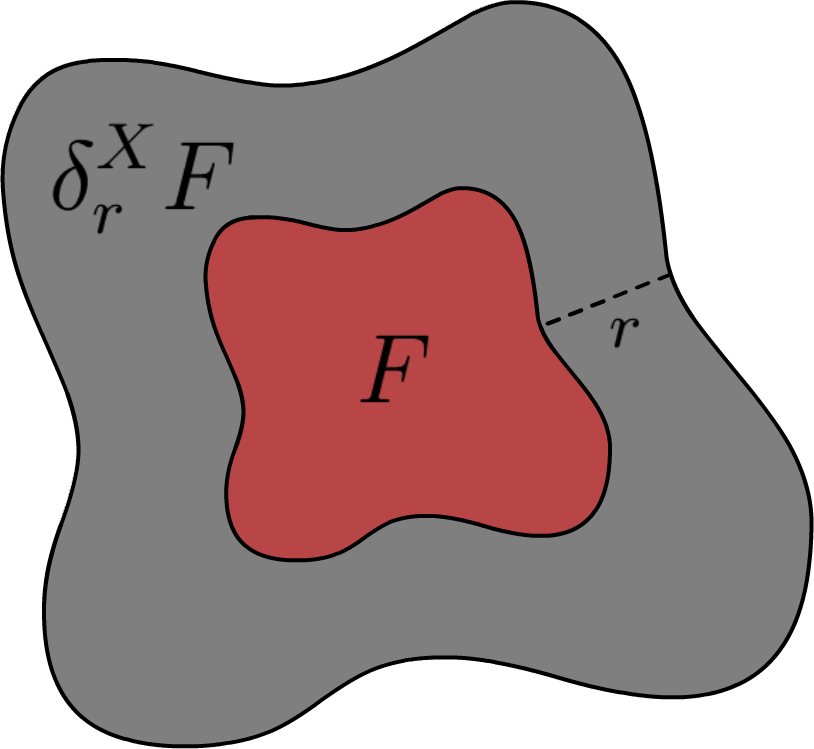
\includegraphics[height=35mm]{rBoundary.png}}
\end{frame}

\begin{frame}
\frametitle{The Many Faces of Amenability}
\begin{corollary}
A group $G$ with finite generating set $S$. If $(G, d_S)$ has subexponential growth -- that is, the size of closed balls of radius $n$ grows no faster than $2^n$ -- then it admits a F{\o}lner sequence and is hence amenable.
\end{corollary}
\end{frame}

\begin{frame}
\frametitle{The Many Faces of Amenability}
\begin{theorem}[Reiter's Property ($P_p$), 1965]
Let $p \in [1, \infty)$. A discrete group $G$ is amenable if and only if, for every finite subset $Q \subset G$ and all $\varepsilon > 0$, there exists some $s \in \ell^p(G)$ such that
\begin{itemize}
\item $s \geq 0$;
\item $\norm{s}_p = 1$;
\item $\norm{q \cdot s - s}_p < \varepsilon$, for all $q \in Q$.
\end{itemize}
\end{theorem}
\noindent\\[0.5\baselineskip]
\begin{theorem}[Hulanicki 1965, Reiter 1966]
A discrete group $G$ is amenable if and only if its universal $C^*$-algebra is equal to its reduced $C^*$-algebra.
\end{theorem}
\end{frame}

\begin{frame}
\frametitle{The Many Faces of Amenability}
\begin{theorem}[Johnson, 1972]
A discrete group $G$ is amenable if and only if $\mathcal{H}^1(\ell^1(G), \chi^*) = \{0\}$ for every Banach $\ell^1(G)$-bimodule $\chi$, where $\mathcal{H}^1$ is the Hochschild cohomology.
\end{theorem}
\noindent\\[0.5\baselineskip]
\begin{theorem}[Bartholdi, 2010]
A group $G$ is amenable if and only if all cellular automata on $G$ that admit mutually erasable patterns also admit a Garden of Eden.
\end{theorem}
\end{frame}

%%%%%%%%%%%%%%
% References %
%%%%%%%%%%%%%%

%\section*{References}

%\begin{frame}[allowframebreaks]
%\frametitle{References}
%\printbibliography[heading = none]
%\end{frame}

%%%%%%%%%%%%%
% Thank you %
%%%%%%%%%%%%%

\begin{frame}
\centerline{\Huge\textcolor{structure}{\underline{Thank you for your attention!}}}
%\vspace*{2em}
%\centerline{\LARGE Any questions?}
\end{frame}

\end{document}